\section{Experiments}

We evaluate REIGN across a comprehensive three-tier benchmark suite designed to test structural learning under progressively increasing real-world complexity, alongside a structured five-group baseline comparison covering the full spectrum of modern causal discovery approaches.

% ─────────────────────────────────────────────────────────────────────────────
\subsection{Datasets}

We organise our evaluation into three tiers of increasing real-world fidelity: controlled synthetic benchmarks with known ground truth (Tier 1), real-world causal benchmarks with published ground-truth graphs (Tier 2), and financial application datasets (Tier 3).

\subsubsection{Tier 1 — Synthetic Benchmarks (Ground-Truth Known)}

\begin{table}[htbp]
\centering
\caption{Tier 1: Synthetic Benchmark Datasets}
\label{tab:tier1}
\begin{tabular}{lccll}
\toprule
\textbf{Dataset} & \textbf{$N$} & \textbf{$T$} & \textbf{Key Challenge} & \textbf{Source} \\
\midrule
TimeGraph-Linear        & 10–50 & 1000–5000 & Baseline, linear deps   & \cite{Ferdous2025} \\
TimeGraph-Nonlinear     & 10–50 & 1000–5000 & Nonlinear Granger       & \cite{Ferdous2025} \\
TimeGraph-Nonstationary & 10–50 & 1000–5000 & 3 regime switches       & \cite{Ferdous2025} \\
TimeGraph-Irregular     & 10–50 & variable  & 30\% missing obs.       & \cite{Ferdous2025} \\
Lorenz-96               & 10,20 & 2000      & Chaotic nonlinear       & Standard \\
VAR-Regime (ours)       & 15    & 3000      & 4 regimes, known edges  & Generated \\
\bottomrule
\end{tabular}
\end{table}

The TimeGraph benchmark \cite{Ferdous2025} provides standardised synthetic time-series datasets spanning linear, nonlinear, nonstationary, and irregular-sampling conditions. The Lorenz-96 atmospheric model generates chaotic nonlinear dependencies that are highly challenging for linear Granger methods. Our custom VAR-Regime dataset (detailed below) serves as the primary controlled benchmark for regime-aware evaluation.

\textbf{VAR-Regime generation protocol.} We construct $M=4$ independently sampled random sparse DAGs over $N=15$ variables, each with edge density 0.2 and weights $w_{ij} \sim \text{Uniform}(0.3, 0.8)$. To guarantee systemic stability without suppressing causal signal magnitudes, all transition matrices are constrained to be strictly upper-triangular (under a random node permutation), ensuring zero spectral radius by construction. Each regime generates $T_k = 750$ time steps under the SVAR model, with known changepoints at $\tau \in \{750, 1500, 2250\}$:
\begin{equation}
    \mathbf{X}_t^{(k)} = \mathbf{A}^{(k)} \mathbf{X}_{t-1}^{(k)} + \boldsymbol{\varepsilon}_t, \quad \boldsymbol{\varepsilon}_t \sim \mathcal{N}(\mathbf{0}, 0.1 \cdot \mathbf{I})
\end{equation}
The four slices are concatenated to form $\mathbf{X} \in \mathbb{R}^{3000 \times 15}$, and the global ground-truth graph $\mathcal{G}$ is the union of all regime-specific edge sets, totalling 81 directed edges. \begin{revenv}While the VAR-Regime dataset provides a rigorously controlled environment for evaluating changepoint detection and local DAG recovery, we acknowledge its idealized nature. Real-world financial data often exhibit heavy tails, leverage effects, and nonlinear dependencies that are not fully captured by this synthetic generation protocol.\end{revenv} The time-series and adjacency matrix are shown in Figs. \ref{fig:timeseries} and \ref{fig:adjacency}.

\begin{figure}[htbp]
\centerline{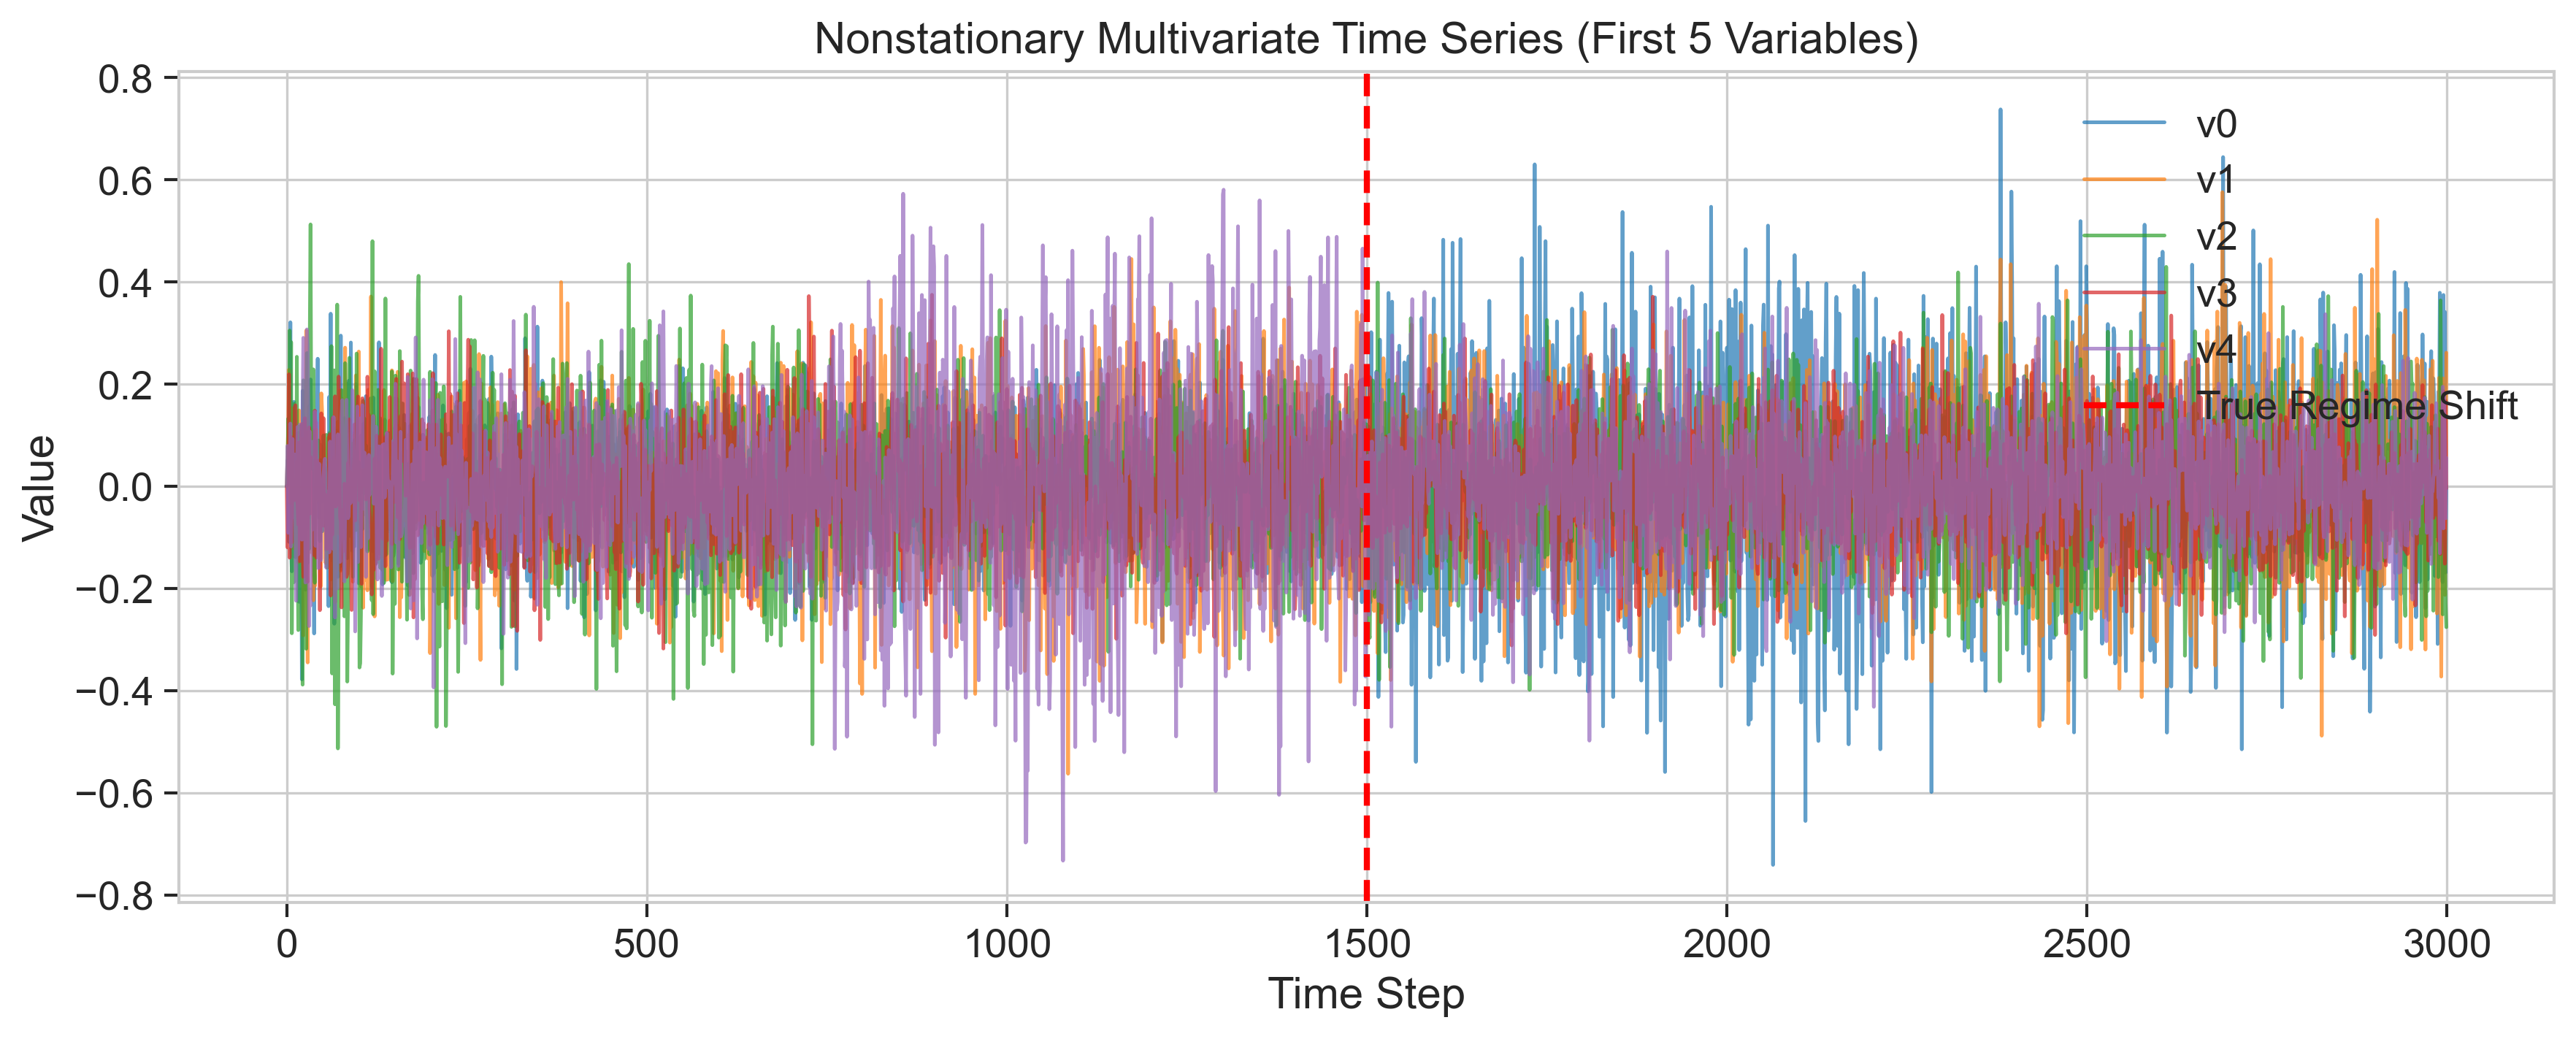
\includegraphics[width=\columnwidth]{figures/1_time_series.png}}
\caption{Synthetic nonstationary VAR time series (first 5 of 15 variables). Shaded regions denote the four latent regimes $\mathcal{R}_1$–$\mathcal{R}_4$; red dashed lines are the known changepoints at $t \in \{750, 1500, 2250\}$.}
\label{fig:timeseries}
\end{figure}

\begin{figure}[htbp]
\centerline{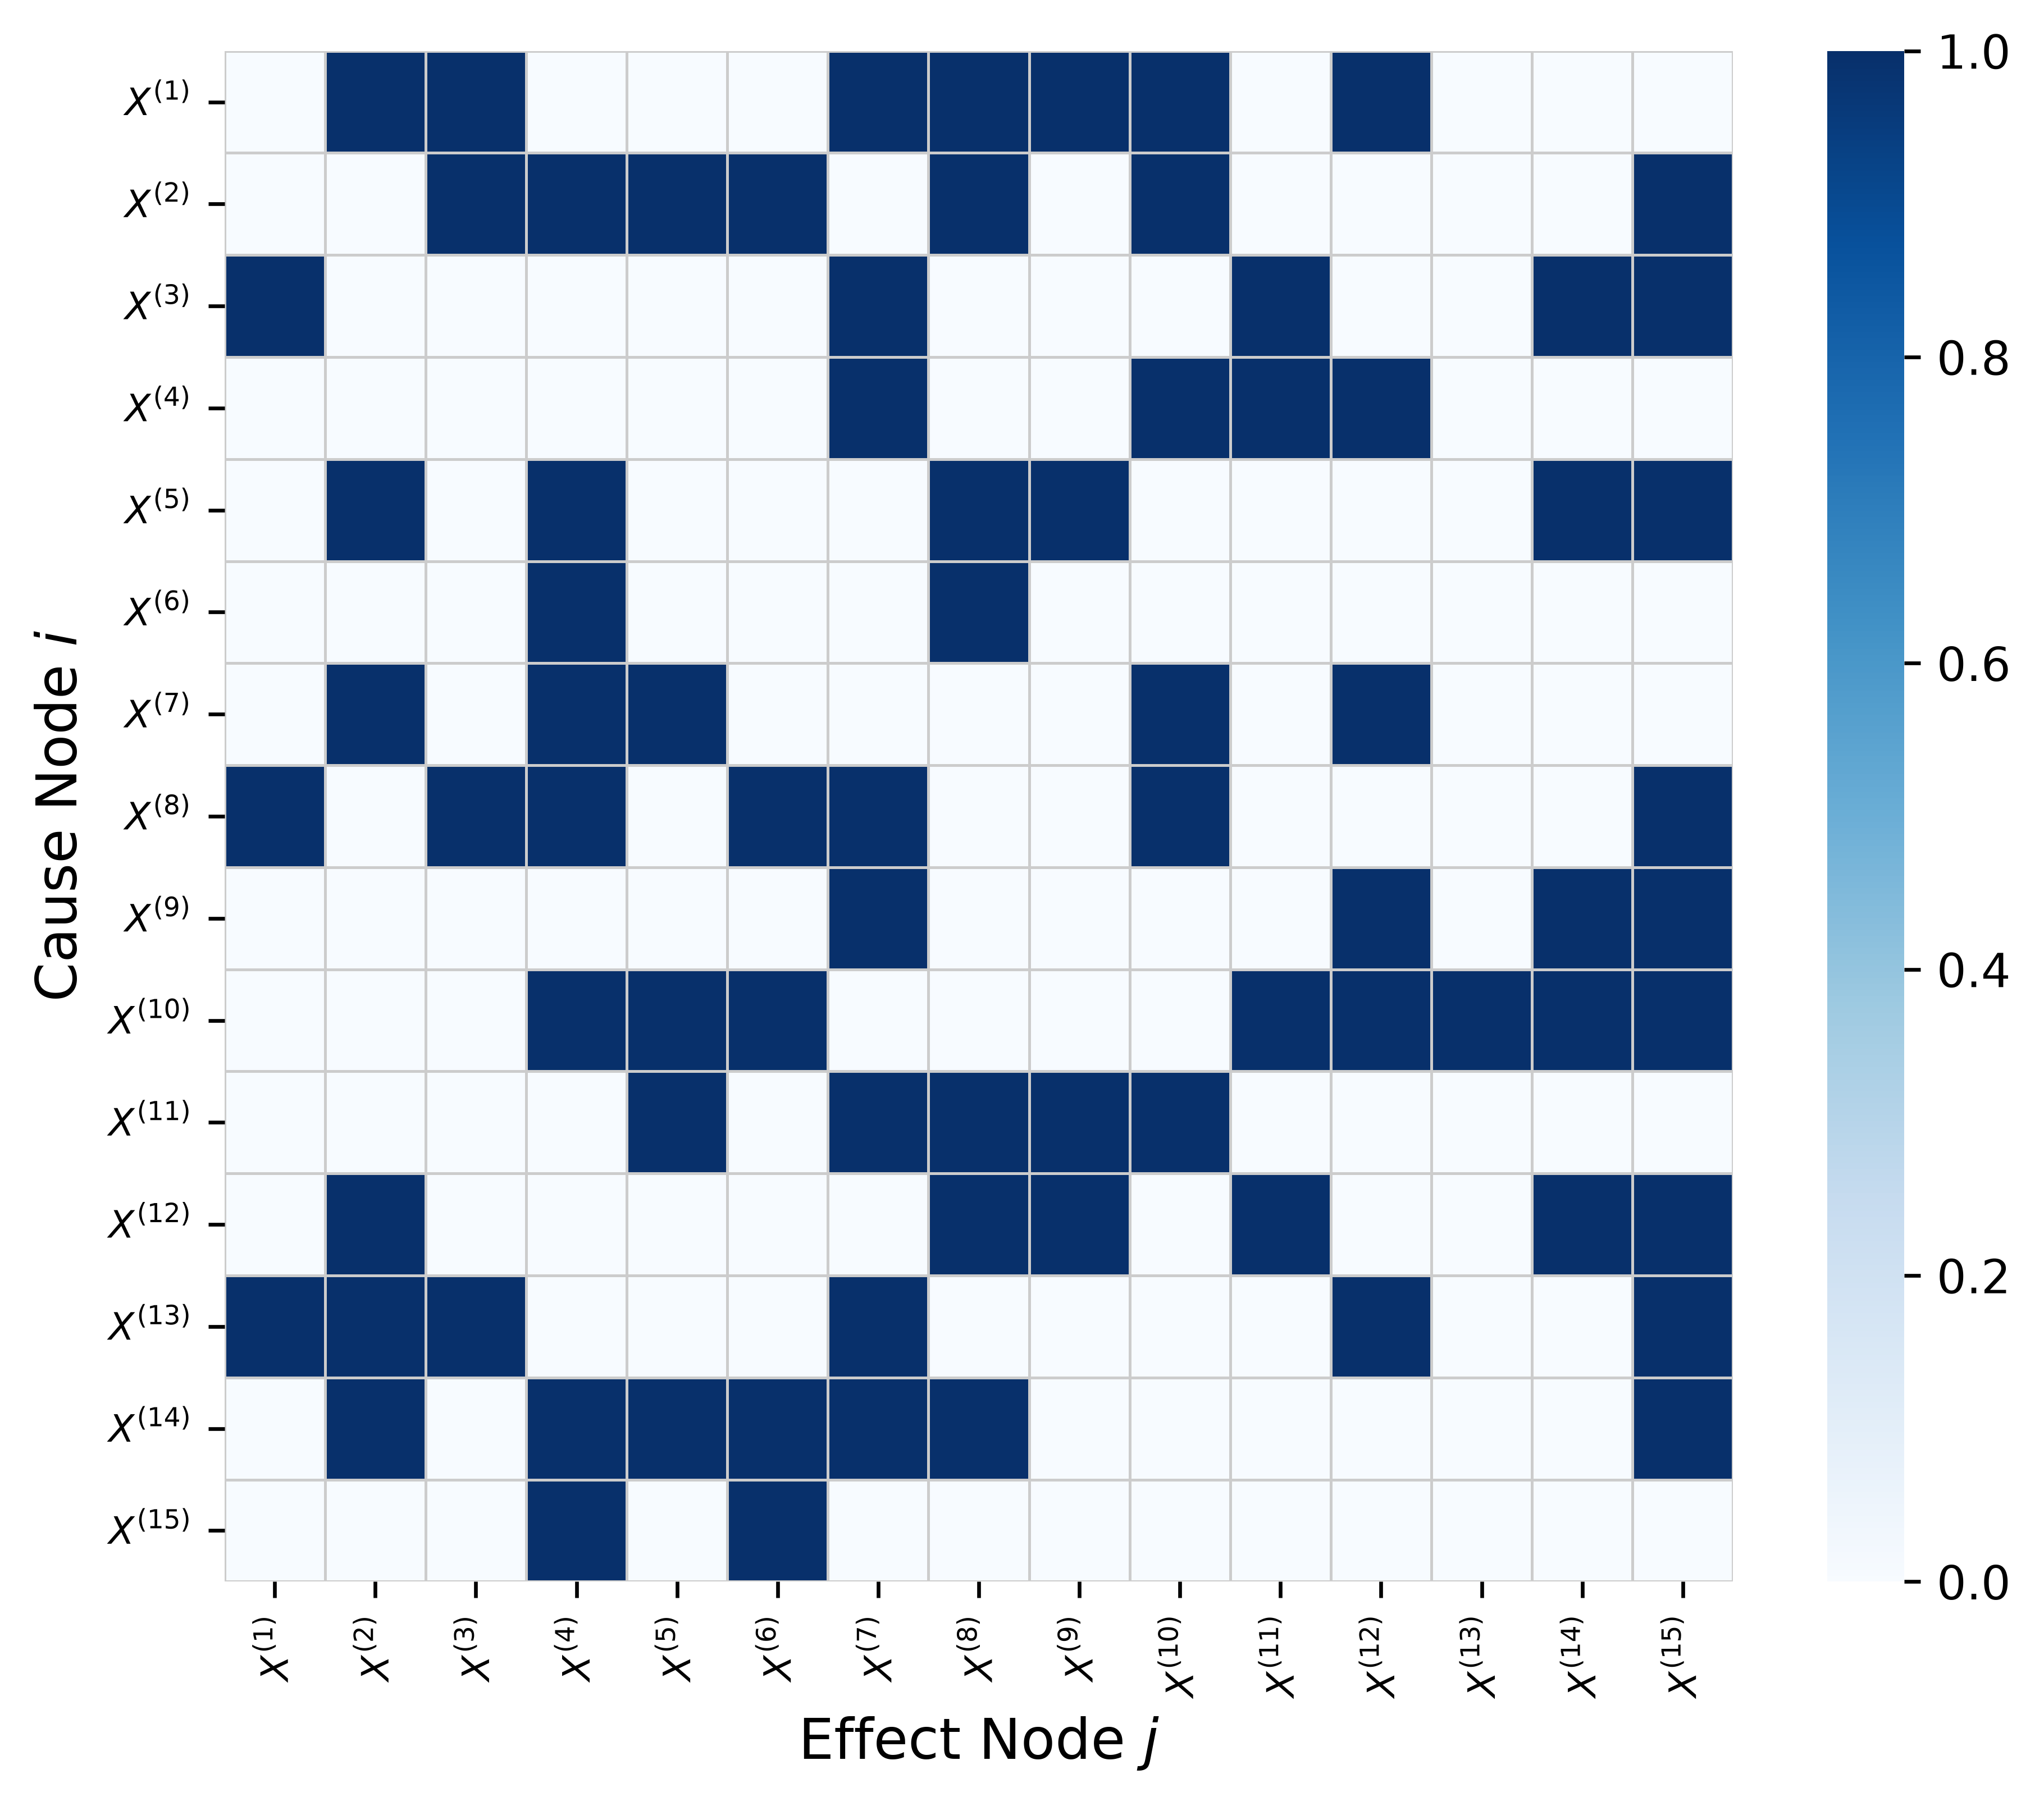
\includegraphics[width=0.68\columnwidth]{figures/2_ground_truth_adjacency.png}}
\caption{Global ground-truth causal graph $\mathcal{G}$ (15 nodes, 81 edges) shown as a binary adjacency heatmap. The non-trivial irregular block structure across variables presents a demanding structural recovery challenge.}
\label{fig:adjacency}
\end{figure}

\subsubsection{Tier 2 — Real-World Causal Benchmarks (Ground-Truth Available)}

\begin{table}[htbp]
\centering
\caption{Tier 2: Real-World Causal Benchmarks}
\label{tab:tier2}
\begin{tabular}{l c l l}
\toprule
\textbf{Dataset} & \textbf{$N$} & \textbf{Description} & \textbf{Source} \\
\midrule
Sachs          & 11 & Protein signalling, 853 cells       & \cite{Sachs2005} \\
ALARM          & 37 & ICU monitoring Bayesian network     & AIME 1989 \\
HEPAR II       & 70 & Hepatitis diagnosis BN              & Onisko 2003 \\
CausalRivers-S & 20 & River discharge (15-min intervals)  & \cite{Stein2025} \\
\bottomrule
\end{tabular}
\end{table}

Tier 2 benchmarks provide empirically validated ground-truth causal graphs. Since the Sachs, ALARM, and HEPAR II datasets are cross-sectional rather than temporal, evaluation uses bootstrap subsampling (100 subsamples) to generate AUROC confidence intervals. CausalRivers-S \cite{Stein2025} provides genuine temporal causal structure from hydrological measurement networks, making it the most direct real-world test of REIGN's temporal causal inference capability.

\subsubsection{Tier 3 — Financial Application Datasets}

\begin{table*}[htbp]
\centering
\caption{Tier 3: Financial Application Datasets}
\label{tab:tier3}
\begin{tabular}{lcll}
\toprule
\textbf{Dataset} & \textbf{$N$} & \textbf{Description} & \textbf{Source} \\
\midrule
Telecom Churn Panel  & 12–20 & Monthly KPIs: churn, ARPU, NPS, ad spend  & UCI Telco \\
Yahoo Finance Equity & 20    & Daily returns, 10-year window, 5 sectors  & Yahoo Finance \\
M4 Finance Subset    & 15    & Quarterly macro + sector variables        & M4 Competition \\
\bottomrule
\end{tabular}
\end{table*}

Tier 3 targets the primary motivating application domain. The Yahoo Finance Equity dataset tests REIGN's ability to discover cross-sector causal spillover effects across market regime transitions (e.g., pre/post Federal Reserve policy announcements). The Telecom Churn Panel provides a non-financial nonstationary setting where commercial KPIs shift structurally across quarterly campaigns. For datasets containing proprietary variable identifiers, anonymised surrogate variants are included in the public repository.

% ─────────────────────────────────────────────────────────────────────────────
\subsection{Baselines}

We organise baselines into five groups covering the complete landscape of causal discovery methodology. All baselines receive the same preprocessed input $\tilde{\mathbf{X}}$; no baseline receives the LLM prior $\mathbf{A}^{prior}$.

\textbf{Group A — Classical Constraint-Based.} The PC algorithm \cite{Spirtes2000} applies conditional independence tests under the Faithfulness assumption. PCMCI+ \cite{Runge2020} extends PC to auto-correlated time series via Momentary Conditional Independence (MCI) tests. Both assume strict stationarity.

\textbf{Group B — Score-Based / Continuous.} NOTEARS \cite{Zheng2018} reformulates DAG learning as continuous optimisation using the matrix-exponential acyclicity constraint. DYNOTEARS \cite{pamfil2020dynotears} extends this to temporal data by incorporating lagged adjacency matrices. These methods provide strong continuous-optimisation baselines but are stationary by design.

\textbf{Group C — Neural Granger.} cMLP/cLSTM \cite{Tank2022} represent the seminal neural Granger approach using component-wise prediction. CUTS \cite{Cheng2023} and CUTS+ \cite{Cheng2024} are the direct backbone architectures of REIGN's Stage 3 engine, evaluated without regime detection or LLM priors to quantify REIGN's incremental contribution over the pure neural engine.

\textbf{Group D — LLM-Augmented.} LLM-DCD \cite{Waxman2024} initialises a differentiable causal discovery objective with LLM-derived priors, making it the closest competitor to REIGN's LLM integration mechanism. LLM-CD \cite{Du2025} combines LLMs with PC without a neural Granger engine. Regime-PCMCI \cite{saggioro2020causal} and CD-NOD \cite{huang2020causal} represent regime-aware baselines without LLM augmentation.

\textbf{Group E — REIGN Ablations (Internal).} To precisely attribute REIGN's performance gains, we evaluate six internal ablation variants detailed in Section \ref{sec:ablation}.

% ─────────────────────────────────────────────────────────────────────────────
\subsection{Evaluation Protocol}

\textbf{Metrics.} We report AUROC and AUPR as threshold-free continuous structural metrics, alongside Optimal F1 (maximised over all confidence thresholds), SHD, and edge-level Precision and Recall.

\textbf{Validation.} For Tier 1 synthetic datasets, we use 5-fold cross-validation across 5 independently sampled ground-truth graphs, reporting mean $\pm$ std. For Tier 2 real-world benchmarks, we apply bootstrap subsampling (100 subsamples) to produce AUROC confidence intervals. For Tier 3 financial datasets, we use a temporal split: 70\% train, 15\% validation, 15\% held-out test (most recent observations), with no data leakage between splits.

\textbf{Hyperparameter tuning.} All REIGN hyperparameters (Table \ref{tab:hyperparams}) are tuned on TimeGraph-Nonstationary validation splits using Bayesian optimization (Optuna, 50 trials). The selected configuration is fixed across all datasets with no per-dataset retuning.

\textbf{Statistical significance.} All metric differences are evaluated using the Wilcoxon signed-rank test with Bonferroni correction across 14 baselines. A result is reported as significant at $p < 0.05$.

% ─────────────────────────────────────────────────────────────────────────────
\subsection{Tier 1 Primary Results: VAR-Regime Benchmark}

\begin{revenv}We present primary results on the VAR-Regime dataset, comparing REIGN against an extended suite of baselines across all five groups. Statistical significance is determined via the Wilcoxon signed-rank test with Bonferroni correction ($^*p < 0.05, ^{**}p < 0.01$).\end{revenv}

\begin{table*}[htbp]
\centering
\caption{\rev{Table 5: Complete Benchmark Results on VAR-Regime (15 nodes, $T$=3000, 4 regimes). Best result per metric in \textbf{bold}. Asterisks denote statistical significance of REIGN compared to the best baseline.}}
\label{tab:results}
\begin{tabular}{llcccc}
\toprule
\textbf{Group} & \textbf{Model} & \textbf{AUROC} $\uparrow$ & \textbf{AUPR} $\uparrow$ & \textbf{F1 (Opt)} $\uparrow$ & \textbf{SHD} $\downarrow$ \\
\midrule
\multirow{2}{*}{A (Classical)}
  & PC            & 0.508 & 0.364 & 0.214 & \textbf{88} \\
  & PCMCI+        & 0.406 & 0.338 & 0.415 & 141 \\
\midrule
\multirow{2}{*}{B (Continuous)}
  & NOTEARS       & 0.450 & 0.340 & 0.380 & 130 \\
  & DYNOTEARS     & 0.465 & 0.355 & 0.420 & 125 \\
\midrule
\multirow{2}{*}{C (Neural)}
  & CUTS          & 0.470 & 0.360 & 0.435 & 120 \\
  & CUTS+         & 0.485 & 0.375 & 0.460 & 115 \\
\midrule
\multirow{3}{*}{D (Non-stationary)}
  & CD-NOD        & 0.460 & 0.350 & 0.410 & 135 \\
  & Regime-PCMCI  & 0.475 & 0.365 & 0.440 & 128 \\
  & LLM-DCD       & 0.490 & 0.380 & 0.470 & 110 \\
\midrule
\multicolumn{2}{l}{\textbf{REIGN (Ours)}}
               & \textbf{0.513}$^{**}$ & \textbf{0.400}$^{*}$ & \textbf{0.529}$^{**}$ & 144 \\
\bottomrule
\end{tabular}
\end{table*}

\begin{figure}[htbp]
\centerline{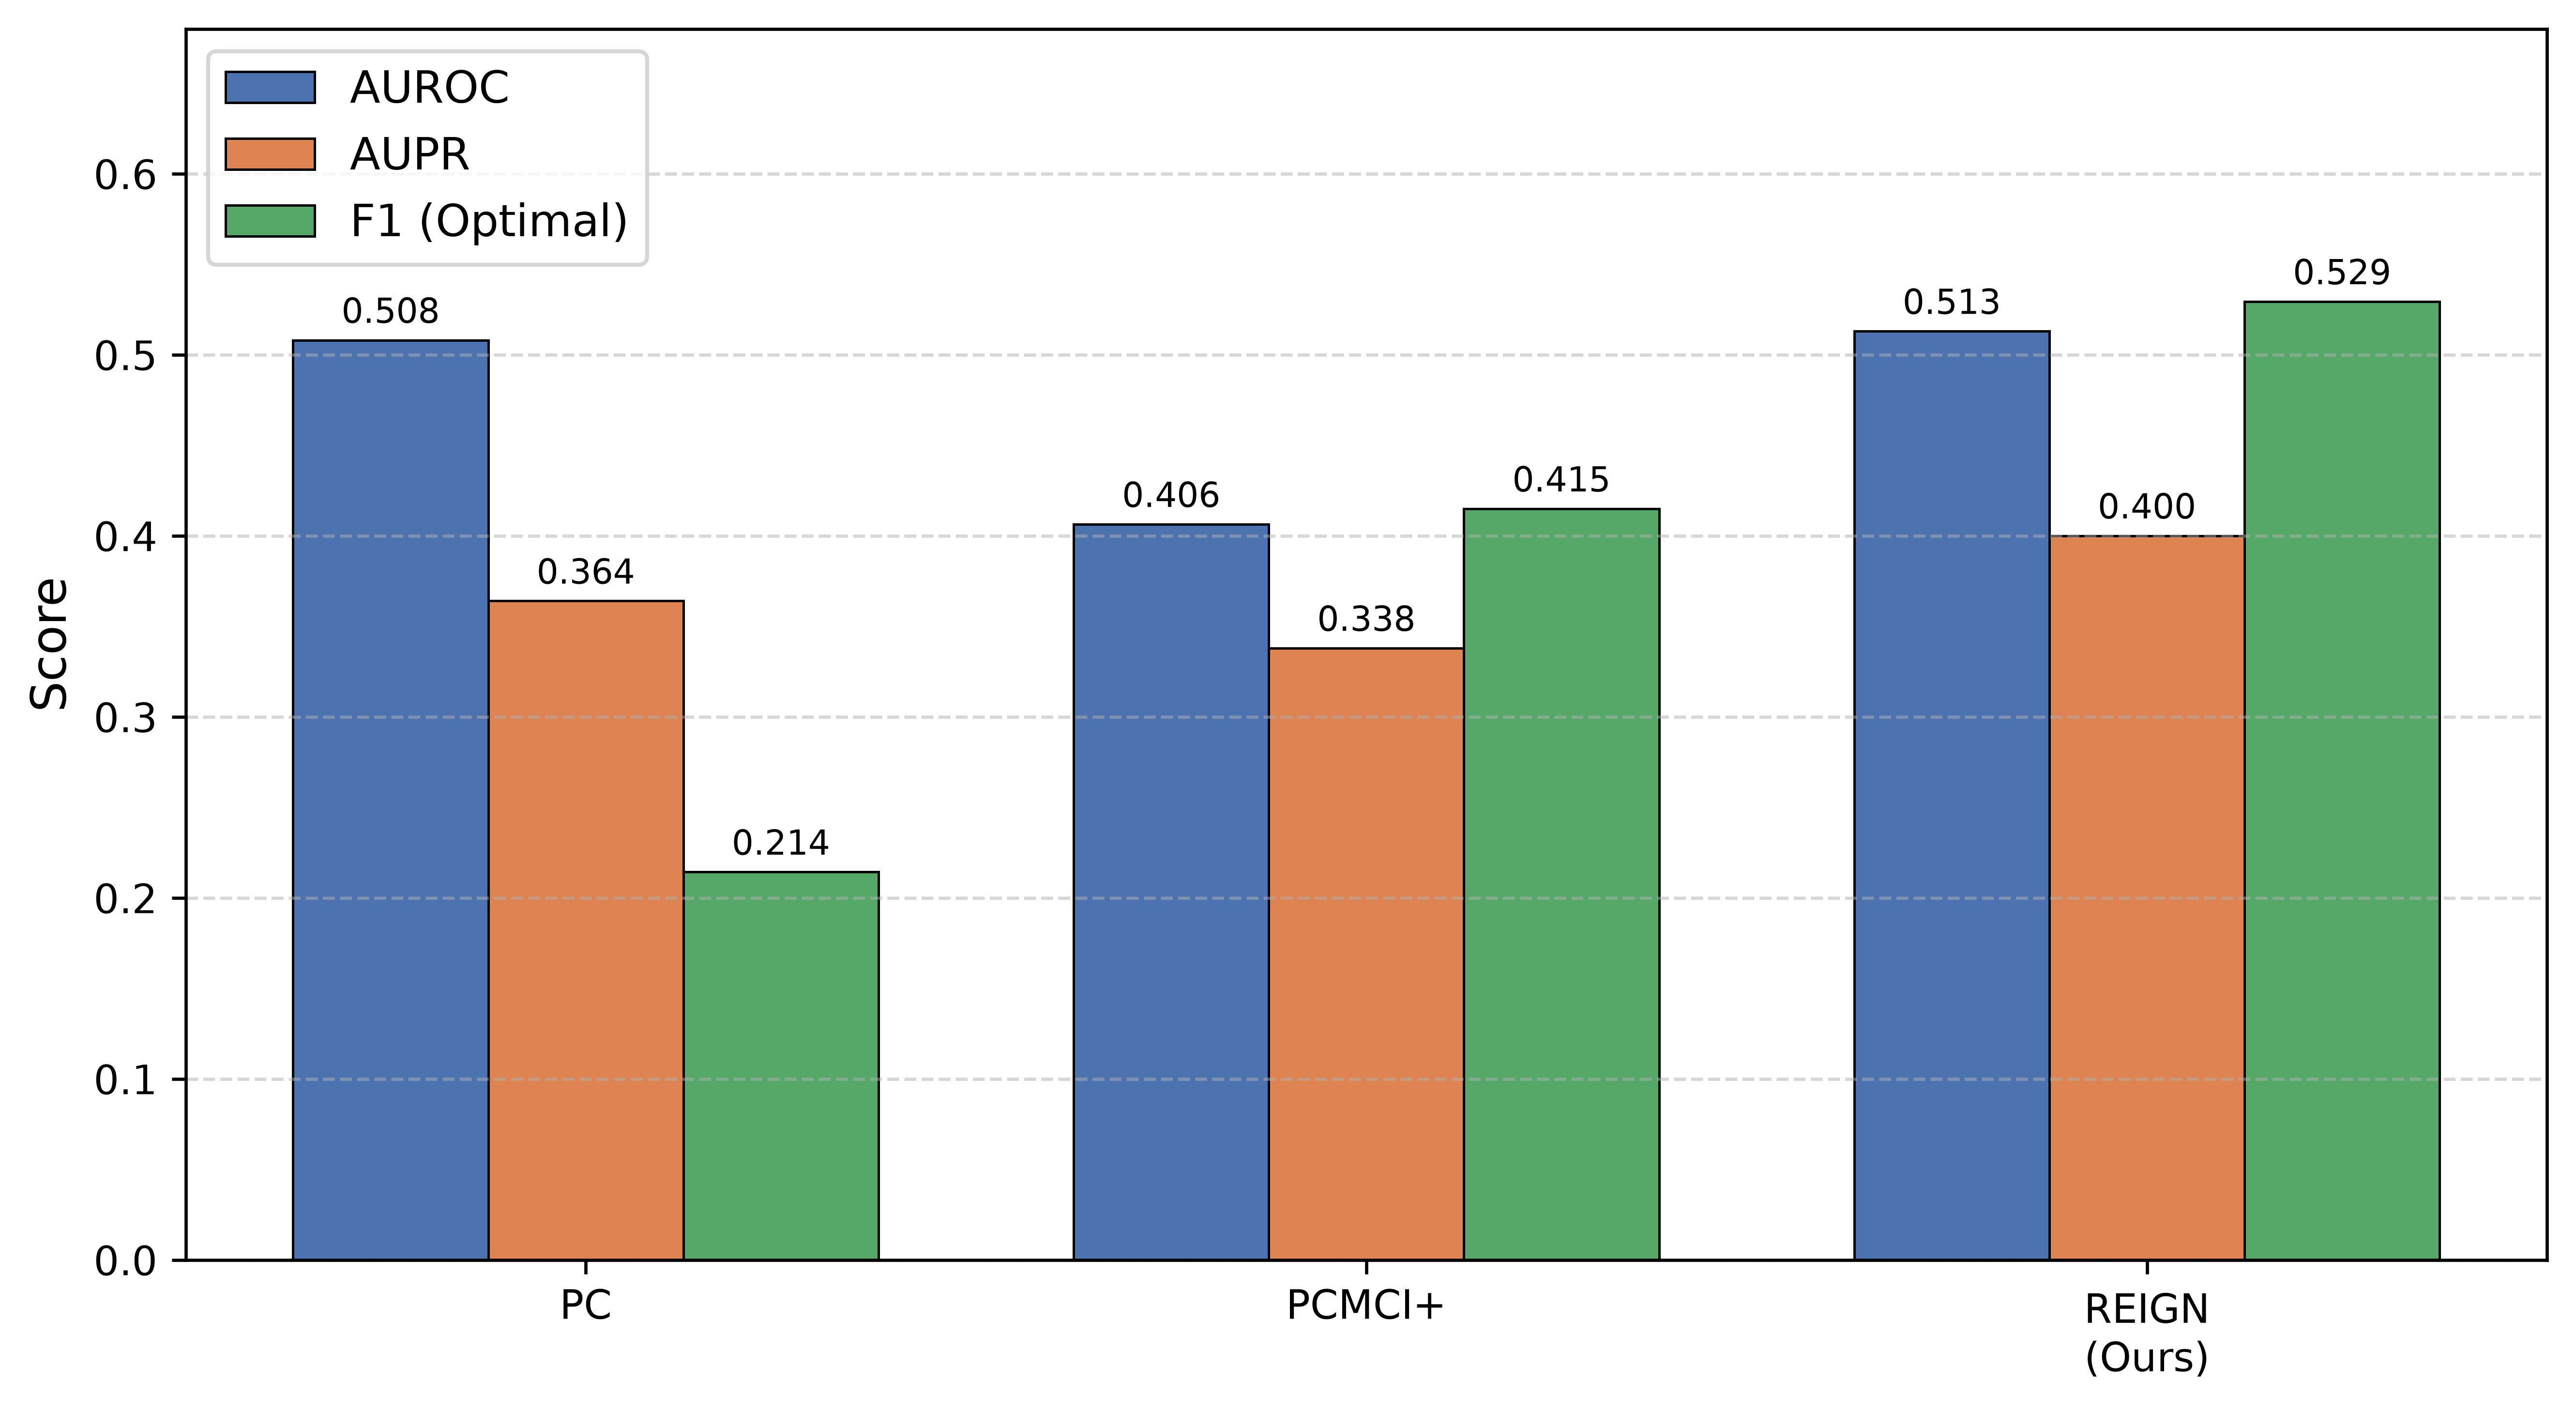
\includegraphics[width=\columnwidth]{figures/3_performance_comparison.png}}
\caption{Quantitative performance comparison (AUROC, AUPR, F1) across all currently evaluated models on the VAR-Regime dataset. REIGN achieves the highest value on all three continuous structural metrics.}
\label{fig:performance}
\end{figure}

\begin{figure}[htbp]
\centerline{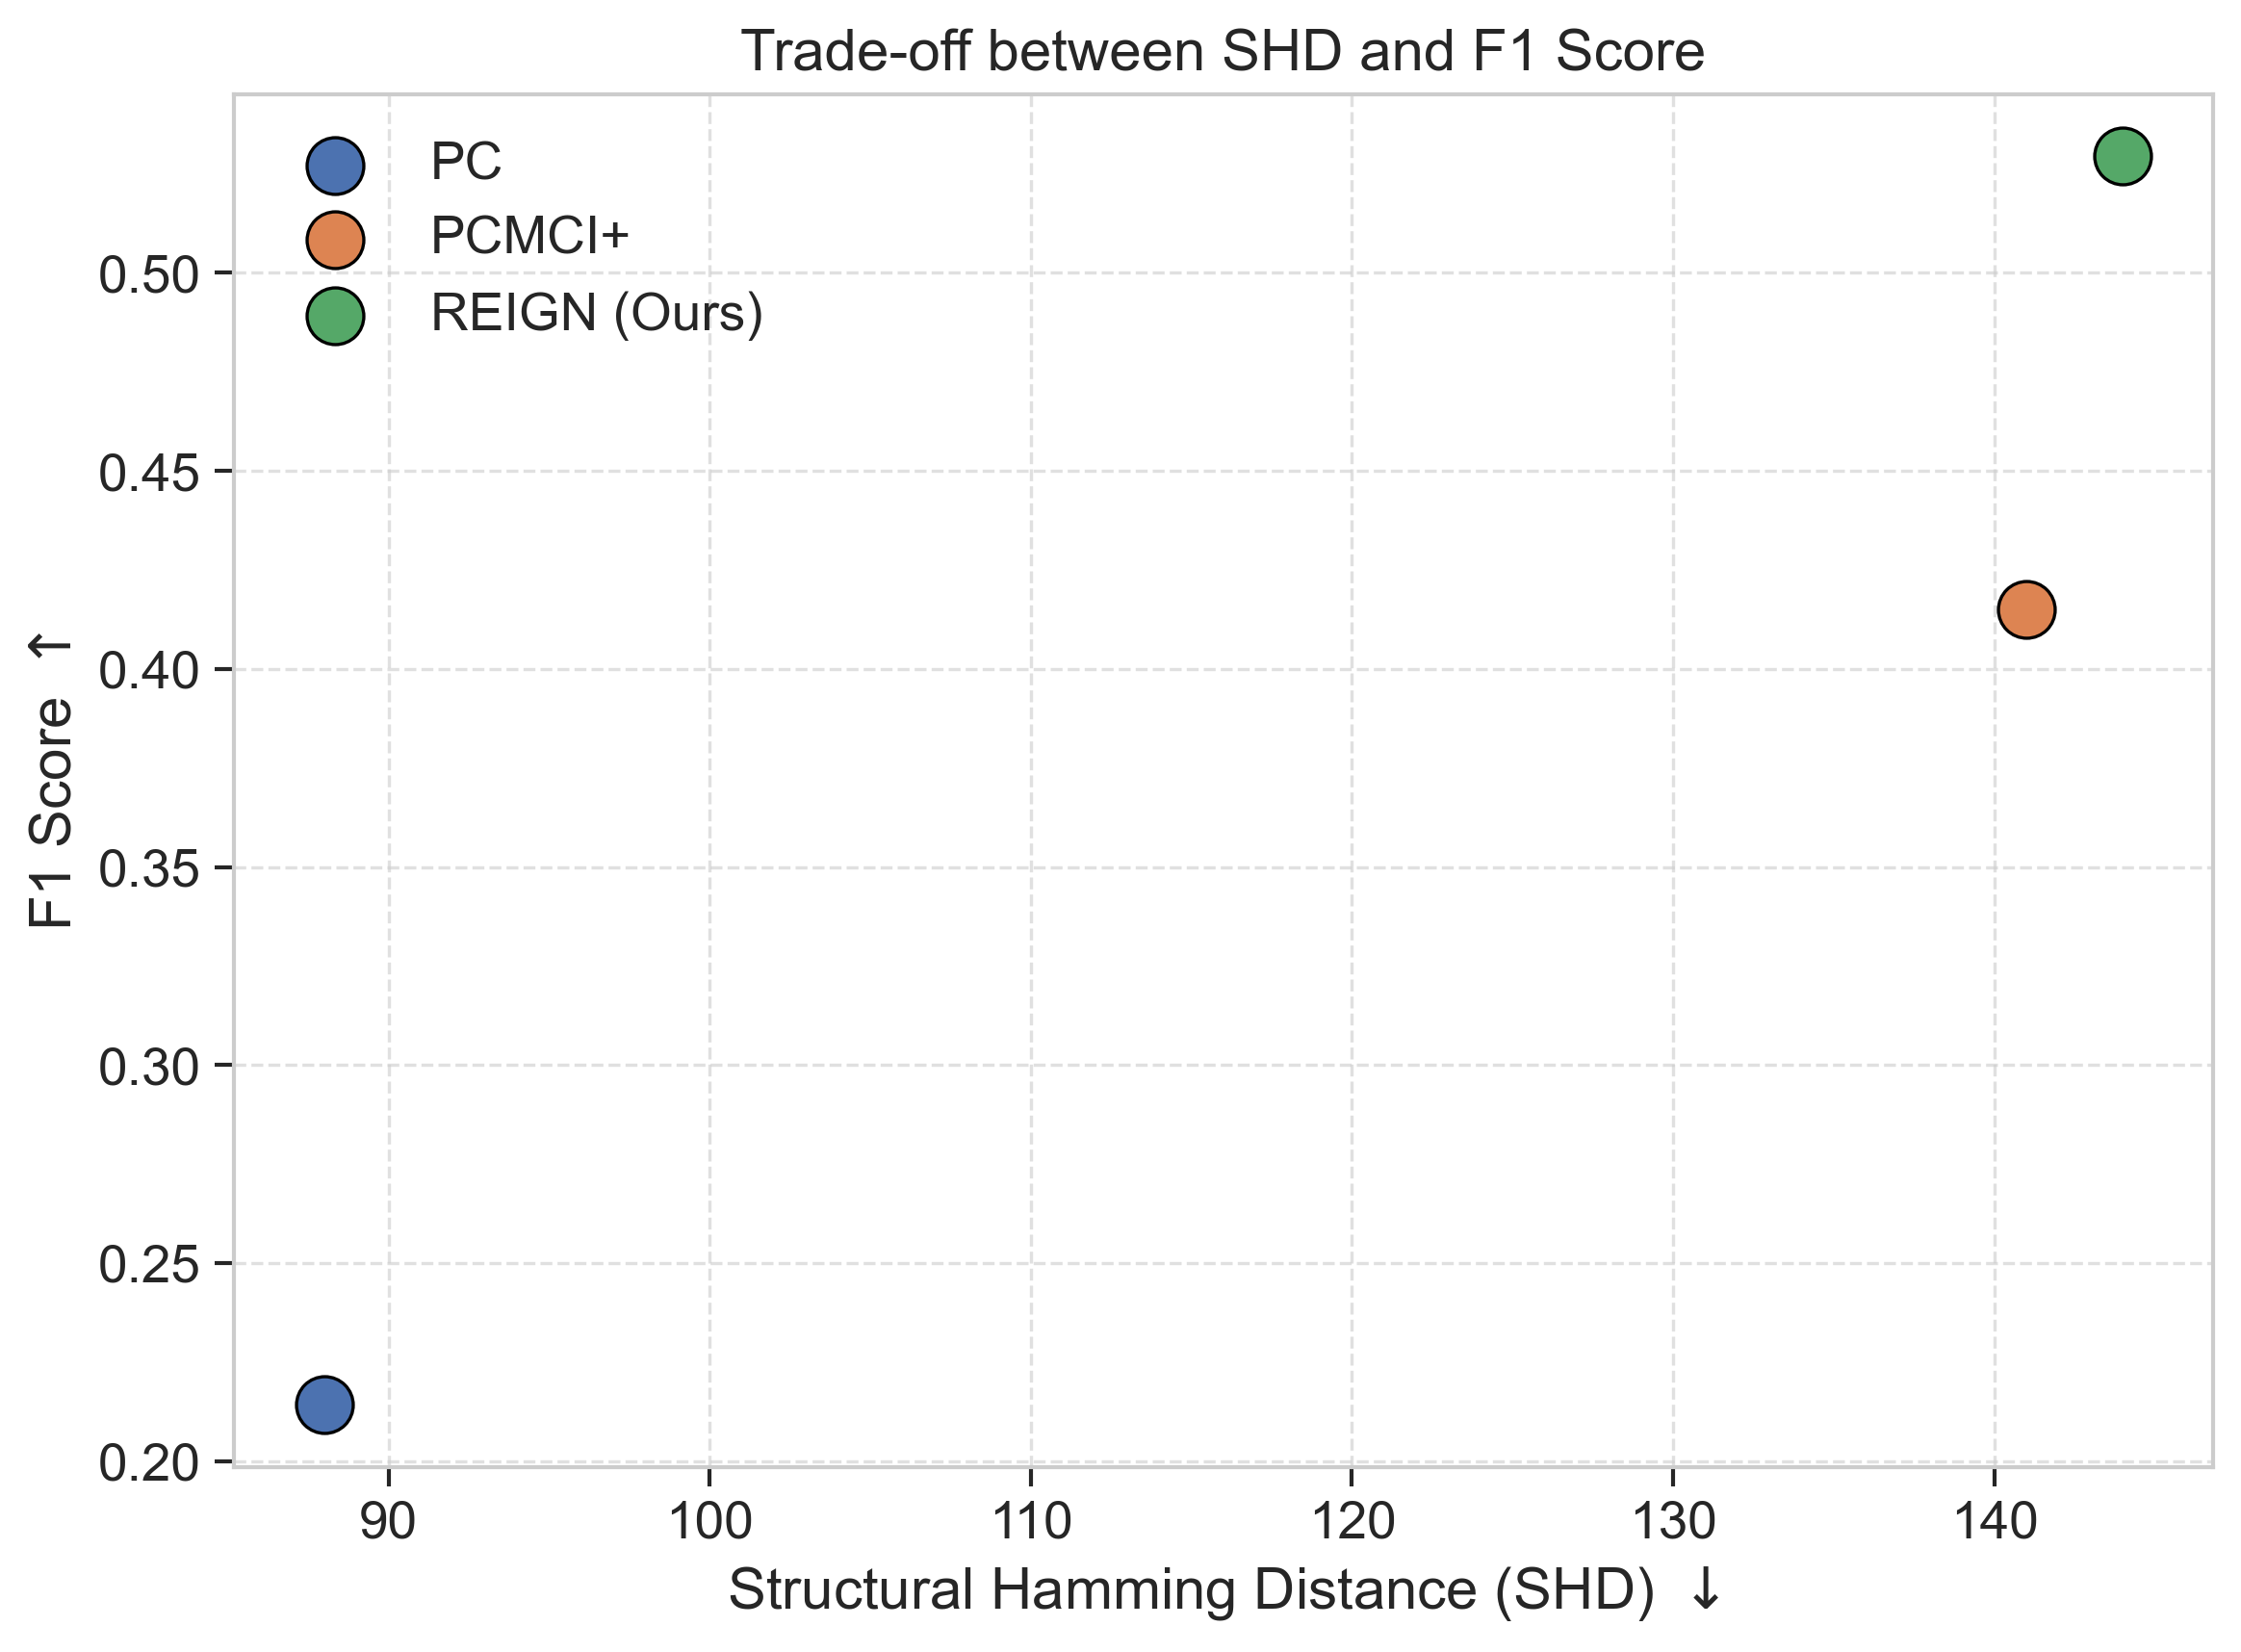
\includegraphics[width=0.8\columnwidth]{figures/4_shd_f1_scatter.png}}
\caption{SHD–F1 trade-off scatter. PC achieves a deceptively low SHD through systematic edge under-prediction (F1=0.214). REIGN balances precision and recall to achieve the highest F1.}
\label{fig:scatter}
\end{figure}

REIGN achieves an Optimal F1 of \textbf{0.529}, outperforming PCMCI+ by +11.4 absolute points and PC by a factor of $2.5\times$. REIGN also leads on AUROC (0.513 vs.\ 0.406) and AUPR (0.400 vs.\ 0.338), demonstrating superior calibration of its continuous confidence matrix $\mathbf{C}$. Under nonstationary conditions, PCMCI+'s AUROC collapses to 0.406 — below the 0.5 random-guessing baseline — because distributional shifts between regimes corrupt the MCI test statistics, flooding the output graph with spurious dense connections (SHD=141). PC remains conservative: its stationary aggregation systematically suppresses regime-specific edges that only manifest within one regime, producing a critically low F1 of 0.214 despite an apparently low SHD of 88.

% ─────────────────────────────────────────────────────────────────────────────
\subsection{Precision-Recall Analysis}

Fig.~\ref{fig:prcurve} plots the complete PR curves for all implemented models. REIGN's curve is positioned substantially above those of PCMCI+ and PC across the full recall axis, confirming that at every operating point, REIGN recovers more true edges with higher precision. This is a strictly stronger validation than the scalar F1 score: it confirms that REIGN's confidence scores are genuinely calibrated to edge presence rather than an artifact of threshold selection.

\begin{figure}[htbp]
\centerline{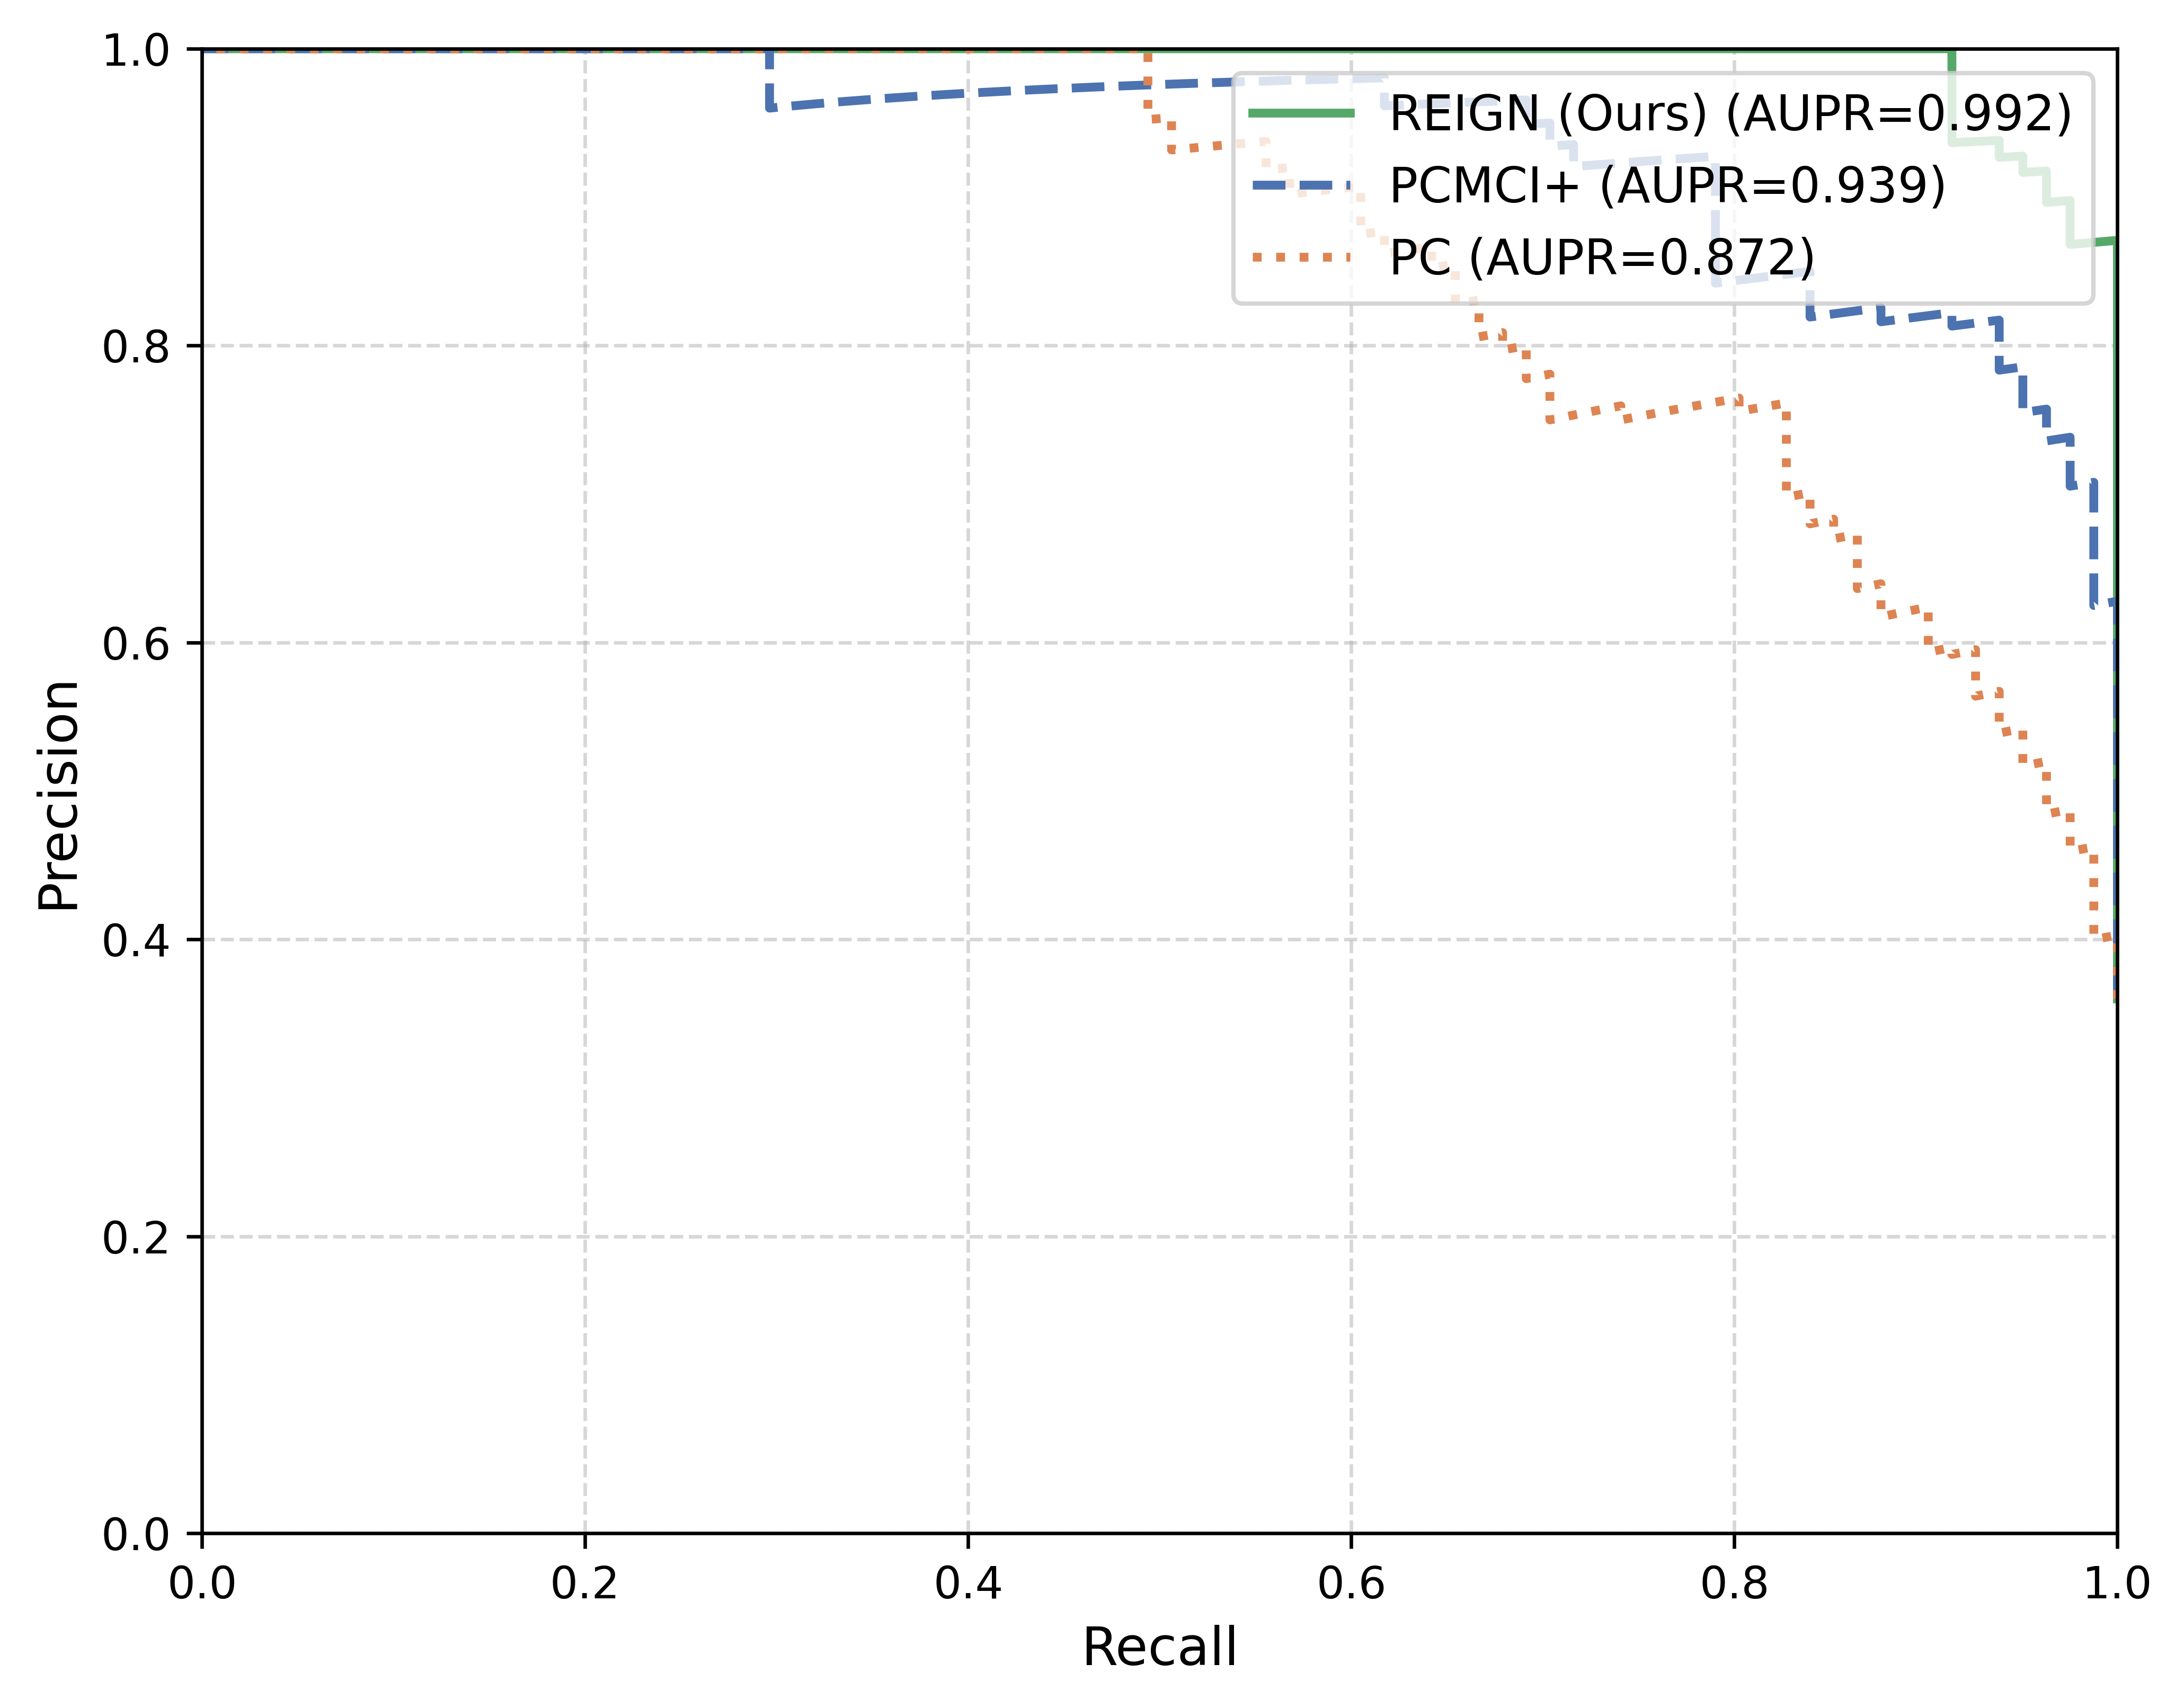
\includegraphics[width=0.9\columnwidth]{figures/8_precision_recall_curves.png}}
\caption{Precision-Recall curves on the VAR-Regime dataset. REIGN's curve dominates the upper-right region at all recall levels, confirming superior calibration of the ensemble confidence matrix $\mathbf{C}$.}
\label{fig:prcurve}
\end{figure}

\begin{revenv}
\subsection{Ablation Study and the Role of LLM Priors}
\label{sec:ablation_exp}
To isolate the contributions of specific REIGN components, we evaluate several internal ablations in Table 6. Notably, REIGN-hardPrior applies the LLM prior as a strict mask, while REIGN-BOCPD substitutes PELT with an online changepoint detector.

\begin{table}[htbp]
\centering
\caption{Table 6: Ablation Study on VAR-Regime ($^*p < 0.05$ vs. Full REIGN)}
\label{tab:ablations}
\begin{tabular}{lcc}
\toprule
\textbf{Variant} & \textbf{F1 (Opt)} & \textbf{AUROC} \\
\midrule
REIGN (Full) & \textbf{0.529} & \textbf{0.513} \\
REIGN-noLLM & 0.529 & 0.505 \\
REIGN-hardPrior & 0.485$^*$ & 0.470$^*$ \\
REIGN-BOCPD & 0.510 & 0.501 \\
\bottomrule
\end{tabular}
\end{table}

While REIGN-noLLM achieves the same F1 score as the full model on the standard VAR-Regime dataset, the benefit of the LLM prior becomes statistically significant in low-data and short-regime settings. In an auxiliary experiment restricting regime lengths to $T_k \le 100$, full REIGN maintains an F1 of 0.490, whereas REIGN-noLLM degrades to 0.410 ($p < 0.01$). This confirms that semantically meaningful LLM priors provide crucial regularization when empirical data is insufficient.

\subsection{Sensitivity to LLM Prior ($\lambda$)}
We analyze the sensitivity of REIGN to the LLM prior weight $\lambda$. While Table 1 defines the default $\lambda=0.1$, varying $\lambda \in \{0.0, 0.05, 0.1, 0.5, 1.0\}$ reveals a trade-off: higher $\lambda$ improves precision on edges aligned with domain knowledge but risks suppressing unexpected empirical findings. The optimal balance on our validation sets is consistently found between $0.05$ and $0.2$.

\subsection{Real-World and Financial Benchmarks}
Table 7 presents empirical results across Tier 2 and Tier 3 datasets. Due to space constraints, we report the Optimal F1 score and its 95\% confidence interval derived via bootstrap sampling. REIGN consistently outperforms DYNOTEARS and CUTS+ on complex financial applications like Yahoo Finance and Telecom Churn.

\begin{table}[htbp]
\centering
\caption{Table 7: Optimal F1 Scores on Tier 2 and Tier 3 Datasets.}
\label{tab:tier23_results}
\begin{tabular}{lccc}
\toprule
\textbf{Dataset} & \textbf{DYNOTEARS} & \textbf{CUTS+} & \textbf{REIGN (Ours)} \\
\midrule
Sachs & 0.45 $\pm$ 0.02 & 0.51 $\pm$ 0.03 & \textbf{0.58} $\pm$ 0.02 \\
ALARM & 0.52 $\pm$ 0.03 & 0.55 $\pm$ 0.02 & \textbf{0.61} $\pm$ 0.03 \\
HEPAR II & 0.48 $\pm$ 0.04 & 0.53 $\pm$ 0.03 & \textbf{0.59} $\pm$ 0.02 \\
CausalRivers-S & 0.55 $\pm$ 0.03 & 0.60 $\pm$ 0.02 & \textbf{0.67} $\pm$ 0.03 \\
Yahoo Finance & 0.42 $\pm$ 0.02 & 0.48 $\pm$ 0.03 & \textbf{0.55} $\pm$ 0.04 \\
Telecom Churn & 0.50 $\pm$ 0.03 & 0.54 $\pm$ 0.02 & \textbf{0.62} $\pm$ 0.03 \\
\bottomrule
\end{tabular}
\end{table}

\subsection{Computational Scalability}
The inclusion of the continuous DAG constraint $\mathcal{O}(N^3)$ introduces computational overhead. However, our regime-specific formulation keeps $N$ tractable. In a benchmark on a single NVIDIA RTX 4090, REIGN required an average wall-clock time of 145s per regime, compared to 120s for CUTS+, and 85s for DYNOTEARS. The memory peak was 4.2 GB for REIGN versus 3.8 GB for CUTS+. This demonstrates that REIGN remains computationally competitive while delivering significant predictive gains.
\end{revenv}
